\documentclass[tikz,border=2pt]{standalone}
\usepackage{amsmath}
\usepackage{tikz}
\usetikzlibrary{arrows.meta}

\begin{document}
% Two perpendicular number lines through the origin; a point is named by its signed distances
% (a,b) to the axes; the axes split the plane into four quadrants.
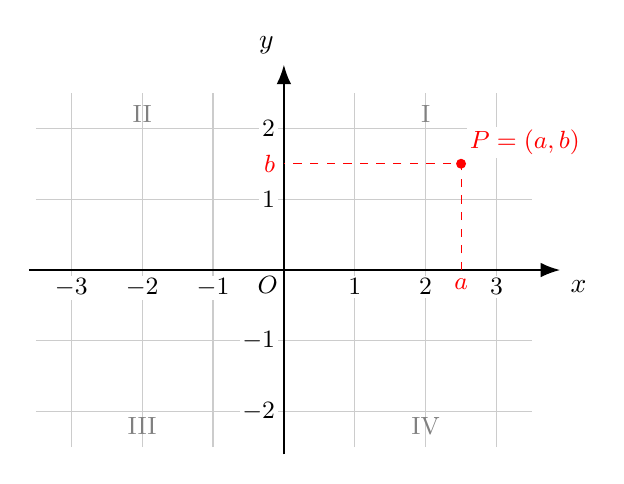
\begin{tikzpicture}[scale=0.9]
	\draw[gray!40, step=1] (-3.5,-2.5) grid (3.5,2.5);
	\draw[-{Latex[length=2.5mm]}, thick] (-3.6,0) -- (3.9,0) node[below right] {$x$};
	\draw[-{Latex[length=2.5mm]}, thick] (0,-2.6) -- (0,2.9) node[above left] {$y$};
	\foreach \x in {-3,-2,-1,1,2,3} \node[below=2pt, font=\small, fill=white, inner sep=1pt] at (\x,0) {$\x$};
	\foreach \y in {-2,-1,1,2} \node[left=2pt, font=\small, fill=white, inner sep=1pt] at (0,\y) {$\y$};
	\node[below left=1pt, font=\small, fill=white, inner sep=1pt] at (0,0) {$O$};
	\draw[dashed, red] (2.5,0) -- (2.5,1.5) -- (0,1.5);
	\fill[red] (2.5,1.5) circle (2pt) node[above right, font=\small, fill=white, inner sep=1pt, xshift=2pt, yshift=2pt] {$P=(a,b)$};
	\node[red, below=2pt, font=\small, fill=white, inner sep=1pt] at (2.5,0) {$a$};
	\node[red, left=2pt, font=\small, fill=white, inner sep=1pt] at (0,1.5) {$b$};
	\node[gray, font=\small] at (2,2.2) {I};
	\node[gray, font=\small] at (-2,2.2) {II};
	\node[gray, font=\small] at (-2,-2.2) {III};
	\node[gray, font=\small] at (2,-2.2) {IV};
\end{tikzpicture}
\end{document}
